\documentclass[tikz,border=3pt]{standalone}
\usetikzlibrary{arrows.meta,calc}
\begin{document}
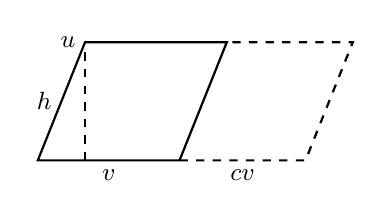
\begin{tikzpicture}[>=Latex, font=\small]
  \coordinate (O) at (0,0);
  \coordinate (U) at (0.6,1.5);
  \coordinate (V) at (1.8,0);
  \coordinate (CV) at (3.4,0);

  \draw[thick] (O) -- (V) -- ($(V)+(U)$) -- (U) -- cycle;
  \draw[thick, dashed] (V) -- (CV) -- ($(CV)+(U)$) -- ($(V)+(U)$);

  \draw[dashed] (0.6,0) -- (U);
  \node[left] at (0.3,0.75) {$h$};

  \node[left] at (U) {$u$};
  \node[below] at ($(O)!0.5!(V)$) {$v$};
  \node[below] at ($(V)!0.5!(CV)$) {$cv$};
\end{tikzpicture}
\end{document}
